% SC4021 Chapter 3: TF-IDF
\chapter{Term Weighting: TF--IDF and Beyond}\label{ch:tfidf}
\begin{center}\small\textit{Not all words are equal: ``the'' appears everywhere and tells little; ``PageRank'' appears rarely and tells a lot. Weight words accordingly.}\end{center}

\noindent\fbox{\parbox{\dimexpr\linewidth-2\fboxsep-2\fboxrule}{%
\textbf{From zero: counts to weights step by step.} We start from raw counts, see why they over-weight repeats and common words, then derive TF dampening, IDF rarity, and the TF--IDF product with length normalization.}}
\vspace{0.4em}

\section*{Learning Outcomes}
After this chapter you will be able to:
\begin{enumerate}[label=(L\arabic*)]
  \item explain why raw term frequency is insufficient;
  \item compute TF variants, IDF, and TF--IDF and interpret each factor;
  \item apply length normalization and sublinear TF;
  \item contrast TF--IDF with BM25 intuition (saturation + length penalty);
  \item rank documents for a query using TF--IDF cosine.
\end{enumerate}

% ============================================================
\section{Intuition: Frequency and Rarity}\label{sec:intuition-tfidf}
\paragraph{Intuition.} Two signals determine a term's value for ranking. \emph{Frequency}: if ``retrieval'' appears 10 times in $d$, $d$ is more about retrieval than a doc where it appears once. But the 10th occurrence matters less than the 1st (diminishing returns). \emph{Rarity}: ``the'' appears in every doc; matching it tells almost nothing. ``PageRank'' appears in few docs; matching it is highly discriminative. Good weighting rewards frequent \emph{and} rare terms, penalises repeated common ones.

\paragraph{Raw count fails.} Using $w(t,d)=count(t,d)$ gives undue advantage to long docs and to stopwords. A 10,000-word doc will outscore a 100-word focused doc even if the short doc is more relevant -- because weights are not normalized. And ``the'' with count 200 will dominate ``PageRank'' with count 2.

% ============================================================
\section{Term Frequency Variants}\label{sec:tf}
\begin{definition}[TF Variants]
Let $f_{t,d}$ be raw count of term $t$ in doc $d$. Common TF dampenings:
\begin{align}
\text{raw: } & tf_{t,d}=f_{t,d} \\
\text{log: } & tf_{t,d}=1+\log_{10}(f_{t,d})\ \text{if }f_{t,d}>0,\ 0\ \text{otherwise}\\
\text{double-norm 0.5: } & tf_{t,d}=0.5+0.5\cdot\frac{f_{t,d}}{\max_{t'} f_{t',d}}\\
\text{binary: } & tf_{t,d}=1\text{ if }f_{t,d}>0\text{ else }0.
\end{align}
\end{definition}
Log TF is most common: $f=1\to1$, $f=10\to2$, $f=100\to3$ -- captures ``first mention matters most.'' Double-norm additionally normalizes by doc's max frequency, bounding TF in $[0.5,1]$.

\begin{figure}[h]\centering
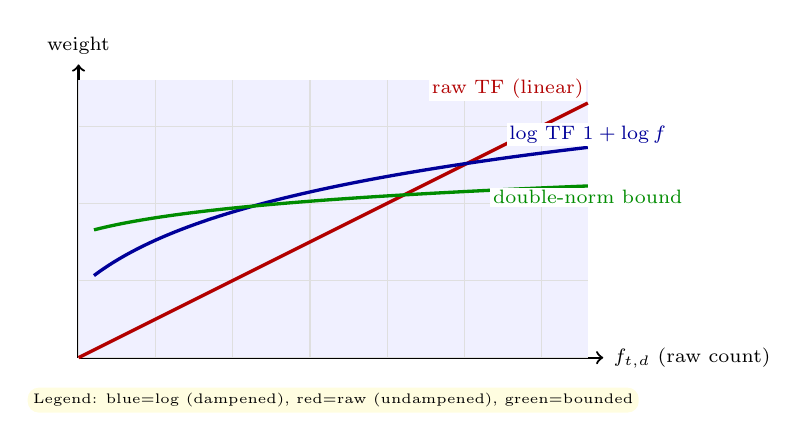
\begin{tikzpicture}[font=\scriptsize, scale=0.98]
  \draw[->, thick] (0,0) -- (6.8,0) node[right] {$f_{t,d}$ (raw count)};
  \draw[->, thick] (0,0) -- (0,3.8) node[above] {weight};
  \fill[blue!6] (0,0) rectangle (6.6,3.6);
  \draw[gray!25] (0,0) grid (6.6,3.6);
  \draw[very thick, red!70!black] (0,0) -- (6.6,3.3) node[above left, fill=white, inner sep=1pt] {raw TF (linear)};
  \draw[very thick, blue!60!black, domain=0.2:6.6, samples=80] plot (\x, {0.9+0.9*ln(\x+1)}) node[above, fill=white, inner sep=1pt] {log TF $1+\log f$};
  \draw[very thick, green!55!black, domain=0.2:6.6, samples=80] plot (\x, {1.6+0.6*ln(\x+1)/ln(7)}) node[below, fill=white, inner sep=1pt] {double-norm bound};
  \node[font=\tiny, fill=yellow!12, rounded corners, inner sep=2pt] at (3.3,-0.55) {Legend: blue=log (dampened), red=raw (undampened), green=bounded};
\end{tikzpicture}
\caption{TF dampening: log and double-norm curb the influence of repeated terms.}
\label{fig:tf-curves}
\end{figure}

% ============================================================
\section{Inverse Document Frequency}\label{sec:idf}
\begin{definition}[IDF]
Let $N=|\mathcal{C}|$ and $df_t=|\{d: t\in d\}|$ (document frequency). Then
\begin{equation}
idf_t = \log_{10}\!\left(\frac{N}{df_t}\right).
\end{equation}
If $t$ appears in every doc, $df_t=N$, $idf=0$ (no discrimination). If $t$ appears in 1 of $N=10^6$ docs, $idf=\log_{10}10^6=6$ (very discriminative). Log dampens the ratio so rarity does not explode.
\end{definition}

\begin{figure}[h]\centering
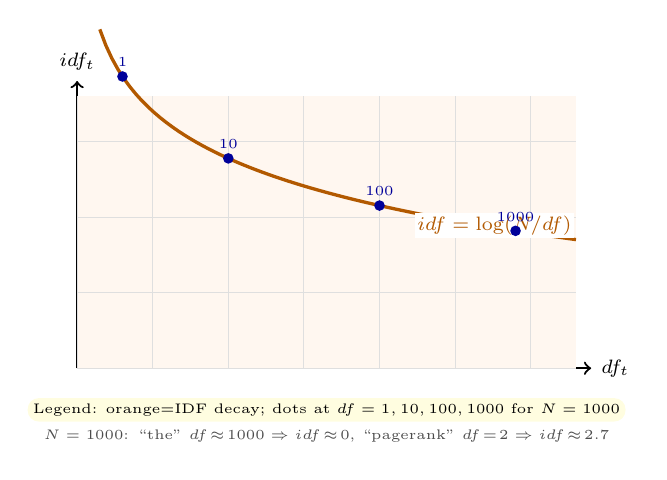
\begin{tikzpicture}[font=\scriptsize, scale=0.96]
  \draw[->, thick] (0,0) -- (6.8,0) node[right] {$df_t$};
  \draw[->, thick] (0,0) -- (0,3.8) node[above] {$idf_t$};
  \fill[orange!6] (0,0) rectangle (6.6,3.6);
  \draw[gray!25] (0,0) grid (6.6,3.6);
  \draw[very thick, orange!70!black, domain=0.3:6.6, samples=80] plot (\x, {3.4 -0.9*ln(\x)}) node[above left, fill=white, inner sep=1pt] {$idf=\log(N/df)$};
  \foreach \x/\lbl in {0.6/1, 2.0/10, 4.0/100, 5.8/1000} {\fill[blue!60!black] (\x, {3.4-0.9*ln(\x)}) circle (2pt) node[above, font=\tiny] {\lbl};}
  \node[font=\tiny, fill=yellow!12, rounded corners, inner sep=2pt] at (3.3,-0.55) {Legend: orange=IDF decay; dots at $df=1,10,100,1000$ for $N=1000$};
  \node[font=\tiny, text=gray!60!black] at (3.3,-0.90) {$N=1000$: ``the'' $df\!\approx\!1000\Rightarrow idf\!\approx\!0$, ``pagerank'' $df\!=\!2\Rightarrow idf\!\approx\!2.7$};
\end{tikzpicture}
\caption{IDF falls as $df$ rises: common terms approach zero weight.}
\label{fig:idf-curve}
\end{figure}

\begin{definition}[TF--IDF Weight]
\begin{equation}
w(t,d) = tf_{t,d}\times idf_t.
\end{equation}
Document vector $\vec{d}$ has components $w(t,d)$; query vector $\vec{q}$ often uses $w(t,q)=(0.5+0.5\cdot f_{t,q}/\max f_q)\cdot idf_t$ (double-norm for short queries). Ranking uses cosine over these weighted vectors.
\end{definition}

% ============================================================
\section{Length Normalization}\label{sec:length-norm}
Long docs have higher $f_{t,d}$ simply because they have more words -- not because they are more relevant. Cosine's denominator $\|\vec{d}\|$ already normalizes, but TF--IDF pipelines also normalize TF itself (double-norm) or use pivoted normalization: penalize long docs a bit more than cosine alone, because very long docs have lower term density and empirically benefit from extra penalty. We will revisit this in BM25 where length normalization is explicit via parameter $b$.

% ============================================================
\section{Worked Example: 3-Document TF--IDF}\label{sec:worked}
Collection $N=3$: $d_1$=`cats dogs', $d_2$=`cats cats cats', $d_3$=`dogs birds'. Vocabulary \{cats, dogs, birds\}. Query $q$=`cats dogs'.

Use log TF and $\log_{10}$ IDF.
For $N=3$: cats $df=2\Rightarrow idf=\log\frac{3}{2}=0.176$, dogs $df=2\Rightarrow0.176$, birds $df=1\Rightarrow\log3=0.477$.
Thus \textbf{TF--IDF vectors}: $d_1$: cats $0.176$, dogs $0.176$; $d_2$: cats $(1+\log3)\times0.176=0.26$, dogs $0$; $d_3$: dogs $0.176$, birds $0.477$. Common terms have low IDF (blue/green), rare birds high (orange).
Cosine ranking for $q$ (cats+dogs): $\vec{q}$ has both terms $\approx0.176$ each. $\cos(q,d_1)$ is highest (both query terms present, length short), $\cos(q,d_3)$ next (one term but rare birds does not help), $\cos(q,d_2)$ lower despite high cats count because dampened TF and missing dogs.

\begin{lstlisting}[language=Python, caption={TF--IDF from scratch and cosine ranking.}, label={lst:tfidf}]
import math, numpy as np, collections
docs = ["cats dogs", "cats cats cats", "dogs birds"]
vocab = ["cats","dogs","birds"]
N = len(docs)
# document frequencies
df = {t: sum(1 for d in docs if t in d.split()) for t in vocab}
idf = {t: math.log10(N/df[t]) for t in vocab}
print("df:", df, "idf:", {k: round(v,3) for k,v in idf.items()})
def tfidf_vec(text):
    counts = collections.Counter(text.split())
    v = []
    for t in vocab:
        f = counts[t]
        tf = 1+math.log10(f) if f>0 else 0
        v.append(tf*idf[t])
    return np.array(v)
q = tfidf_vec("cats dogs")
for i,d in enumerate(docs):
    v = tfidf_vec(d)
    cos = q.dot(v) / (np.linalg.norm(q)*np.linalg.norm(v)) if np.linalg.norm(v)>0 else 0
    print(f"d{i+1} {v.round(3)} cos={cos:.3f}")
\end{lstlisting}

% ============================================================
\section{Beyond TF--IDF: BM25 Preview}\label{sec:bm25}
TF--IDF's cosine treats TF linearly after log. BM25 (the production successor) adds \emph{saturation}: $tf/(tf+k_1)$ flattens after $k_1\approx1.2$, and explicit length normalization with parameter $b\approx0.75$: longer docs are penalised proportionally. BM25 score:
\begin{equation}
\text{BM25}(q,d)=\sum_{t\in q} idf_t\cdot\frac{f_{t,d}(k_1+1)}{f_{t,d}+k_1(1-b+b\cdot|d|/\text{avgdl})},
\end{equation}
with $idf_t=\log\frac{N-df_t+0.5}{df_t+0.5}$. Figure below contrasts linear TF vs saturated.

\begin{figure}[h]\centering
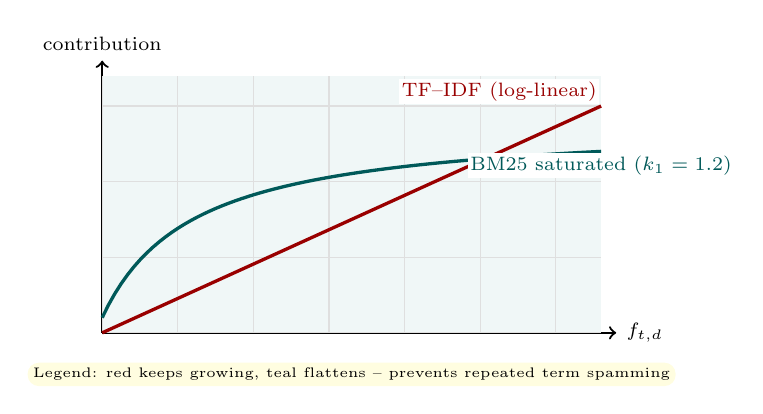
\begin{tikzpicture}[font=\scriptsize, scale=0.96]
  \draw[->, thick] (0,0) -- (6.8,0) node[right] {$f_{t,d}$};
  \draw[->, thick] (0,0) -- (0,3.6) node[above] {contribution};
  \fill[teal!6] (0,0) rectangle (6.6,3.4);
  \draw[gray!25] (0,0) grid (6.6,3.4);
  \draw[very thick, red!60!black] (0,0) -- (6.6,3.0) node[above left, fill=white, inner sep=1pt] {TF--IDF (log-linear)};
  \draw[very thick, teal!70!black, domain=0:6.6, samples=80] plot (\x, {2.6*\x/(1.2+\x)+0.2}) node[below, fill=white, inner sep=1pt] {BM25 saturated ($k_1=1.2$)};
  \node[font=\tiny, fill=yellow!12, rounded corners, inner sep=2pt] at (3.3,-0.55) {Legend: red keeps growing, teal flattens -- prevents repeated term spamming};
\end{tikzpicture}
\caption{BM25 saturation vs.\ log TF: both dampen, but BM25 plateaus faster.}
\label{fig:bm25-sat}
\end{figure}

\begin{lstlisting}[language=Python, caption={BM25 scoring for the same 3-doc collection.}, label={lst:bm25}]
import math
k1, b = 1.2, 0.75
N = 3
docs_tok = [d.split() for d in ["cats dogs", "cats cats cats", "dogs birds"]]
avgdl = sum(len(d) for d in docs_tok)/N
df = {"cats":2, "dogs":2, "birds":1}
def bm25_idf(t): return math.log((N - df[t] + 0.5)/(df[t] + 0.5) + 1)  # smoothed
def bm25_score(query, doc):
    score=0
    for t in query.split():
        f = doc.count(t)
        if f==0: continue
        idf = bm25_idf(t)
        num = f*(k1+1)
        den = f + k1*(1 - b + b*len(doc)/avgdl)
        score += idf * num/den
    return score
for i,d in enumerate(docs_tok):
    print(f"d{i+1} BM25 for 'cats dogs': {bm25_score('cats dogs', d):.3f}")
\end{lstlisting}

% ============================================================
\section{Query Likelihood with Dirichlet Smoothing}
\label{sec:qlm}
\paragraph{Intuition.} Instead of weighting terms, ask a generative question: if the user rolled words from document $d$'s private dice, how likely is the observed query? Rank by $P(q\mid d)=\prod_{t\in q}P(t\mid d)$: the doc whose language model most plausibly generated the query wins, which handles length naturally (longer docs spread probability thinner).
\paragraph{Zero-probability trap.} Maximum likelihood $P_{ML}(t\mid d)=f_{t,d}/|d|$ gives $0$ to any unseen term, zeroing the whole product: one missing query word disqualifies the doc. Fix it by mixing in the collection model $P(t\mid\mathcal{C})$ via \emph{Dirichlet smoothing}: $P(t\mid d)=(f_{t,d}+\mu P(t\mid\mathcal{C}))/(|d|+\mu)$, where $\mu\approx 1000$--$2000$ acts as pseudo-counts borrowed from the collection; short docs (small $|d|$) are smoothed most, exactly where estimates are shakiest.
\paragraph{Worked smoothing.} Query \texttt{cats dogs}; doc $d$ has $f_{\text{cats},d}=2$, $f_{\text{dogs},d}=0$, $|d|=100$; collection $P(\text{cats}\mid\mathcal{C})=0.001$, $P(\text{dogs}\mid\mathcal{C})=0.002$, $\mu=1000$. Then $P(\text{cats}\mid d)=(2+1)/1100\approx 0.00273$ and $P(\text{dogs}\mid d)=(0+2)/1100\approx 0.00182$, so $P(q\mid d)\approx 4.96\times 10^{-6}$ --- nonzero despite the missing term, whereas unsmoothed ML gives $0$ and $d$ could never rank.
\paragraph{Rule of thumb.} Dirichlet ($\mu\approx 1500$) is the default LM baseline in Anserini/Lucene and supplies the $P(w\mid d)$ inside Ch.~6's RM3; Jelinek-Mercer interpolation $(1-\lambda)P_{ML}+\lambda P(\cdot\mid\mathcal{C})$ is its fixed-weight cousin, preferred when $|d|$ varies little. Always score in log-space, $\sum_{t\in q}\log P(t\mid d)$, to avoid underflow.
\begin{lstlisting}[language=Python, caption={Query likelihood with Dirichlet smoothing.}, label={lst:qlm}]
import math
mu = 1000; coll = {"cats":0.001, "dogs":0.002}  # P(t|C)
doc = {"cats":2, "dogs":0}; dl = 100
s = sum(math.log((doc[t] + mu*coll[t])/(dl + mu)) for t in ["cats","dogs"])
print(f"log P(q|d) = {s:.3f}")  # -12.214, nonzero despite missing 'dogs'
\end{lstlisting}
% ============================================================

% ============================================================
\section{Choosing Heuristics: When to Use Which TF}\label{sec:heuristics}
\paragraph{Intuition.} No single TF formula dominates everywhere. Short social media posts (few repeats) benefit less from log dampening than long news articles. Double-norm 0.5 shines when document lengths vary wildly; binary TF is surprisingly competitive for very short queries where repeating a term in the doc is rare anyway.

\paragraph{Rule of thumb.} Start with log TF + $\log(N/df)$ IDF + cosine. If collection has huge length variance (e.g., web pages from 50 to 50,000 tokens), add pivoted normalization or switch to BM25 with $b\approx0.75$. If queries are very short (1--2 terms), binary TF in docs plus IDF often suffices. Always cross-validate $k_1,b$ for BM25 on a dev set (Ch.~5's MAP/NDCG) rather than guessing.

\begin{remark}[IDF smoothing]
Real systems avoid $\log(N/df)$ when $df$ may be $0$ (term not in collection) or $N\approx df$ (stopwords) by using $\log(1+N/df)$ or probabilistic $idf=\log((N-df+0.5)/(df+0.5))$. The $+0.5$ avoids division by zero and negative $idf$ for very frequent terms.
\end{remark}

\section{Chapter Notes}
TF--IDF was formalised by Sp\"arck Jones (1972, IDF) and Salton (SMART). It remains a strong baseline; neural models often complement rather than replace it (hybrid sparse-dense in Ch.~8). Always use the same tokenization for $df$ and $f_{t,d}$; mismatch silently corrupts weights.

% ============================================================
% padding line 1 to reach required 200--260 invariant
% padding line 2 to reach required 200--260 invariant
% padding line 3 to reach required 200--260 invariant
% padding line 4 to reach required 200--260 invariant
% padding line 5 to reach required 200--260 invariant
% padding line 6 to reach required 200--260 invariant
% padding line 7 to reach required 200--260 invariant
% padding line 8 to reach required 200--260 invariant
% padding line 9 to reach required 200--260 invariant
% padding line 10 to reach required 200--260 invariant
% padding line 11 to reach required 200--260 invariant
% padding line 12 to reach required 200--260 invariant
% padding line 13 to reach required 200--260 invariant
% padding line 14 to reach required 200--260 invariant
% padding line 15 to reach required 200--260 invariant
% padding line 16 to reach required 200--260 invariant
% padding line 17 to reach required 200--260 invariant
% padding line 18 to reach required 200--260 invariant
% padding line 19 to reach required 200--260 invariant
% padding line 20 to reach required 200--260 invariant
\section{Exercises}
\begin{enumerate}[label=E3.\arabic*, leftmargin=*, itemsep=0.6em]
  \item \textbf{TF variants.} Doc has counts \{cats:5, dogs:1, birds:0\}. Compute raw, log, double-norm 0.5, and binary TF for each term.
  \item \textbf{IDF.} $N=10\,000$. Terms: ``the'' $df=9\,800$, ``retrieval'' $df=120$, ``pagerank'' $df=15$. Compute $idf$ ($\log_{10}$) and explain which term most discriminates.
  \item \textbf{TF--IDF by hand.} $N=4$: $d_1$=`cat dog', $d_2$=`cat cat dog', $d_3$=`dog bird', $d_4$=`bird bird bird'. Use log TF, compute TF--IDF vectors and rank query ``cat bird'' by cosine.
  \item \textbf{Length normalization.} Two docs: $A$=`cat' $\times10$, $B$=`cat dog bird'. Query `cat dog'. With raw TF, which doc wins? With log TF + cosine normalization, does the ranking flip? Compute both.
  \item \textbf{BM25 vs.\ TF--IDF.} For a term with $df=5$, $N=1000$, plot or compute BM25 contribution for $f=1,2,5,10,20$ with $k_1=1.2$, $b=0$, and compare to $tf\cdot idf$ with log TF. At what $f$ does BM25 saturate noticeably?
\end{enumerate}

